%%%%%%%%%%%%%%%%%%%%%%%%%
%                                                     %
%                      Experiment M-04                %
%         Experiment Title:  Centripetal Force        %
%                                                     %
%%%%%%%%%%%%%%%%%%%%%%%%%

\labChapter{M}{Centripetal Force with Mass on Rotating Arm}
\label{lab:M4}

% Introduction
%\section{Introduction}


% Background
\section{Background}

Acceleration is the measure of the rate of change of the velocity of an object by an external force.  An object moving in a circle with radius $R$ is always being accelerated, even if its speed does not change.  Since velocity is a vector quantity, a centripetal force is required to change its direction. The radial centripetal acceleration, towards the axis of the rotational motion, has magnitude $\nicefrac{v^{2}}{R}$.  The force producing this acceleration on an object of mass $m$ will then have a magnitude of $m v^{2} / R$.

In this experiment, this centripetal force is measured for an object in circular motion while varying the object's speed.  The centripetal force is supplied by a string pulling on the mass in an inwardly radial direction and is then measured by a force sensor (PASCO stated resolution of 0.002 N).



An object in uniform circular motion requires a centripetal or center-seeking force to change the direction of velocity vector.  This centripetal force is related quadratically to the speed of the object, and inversely to its radius of curvature.  As derived in your text, the magnitude of this force acting on an object of mass $m$ with a radius of curvature $R$, is given by
\begin{equation}
  F_{c} = m \frac{v^2}{R}
\end{equation}

During each experiment the mass $m$ and the radius $R$ are fixed by attaching a small weight to a holder on a rotating arm as shown in Fig.~\ref{M04Fig01}. By measuring the force in the cable and the speed of the attached mass on the rotating arm, the mass $m$ can be determined from a graph of force $F$ vs.\ $v^2$.

%Figure01
\begin{figure}
  \begin{center}
    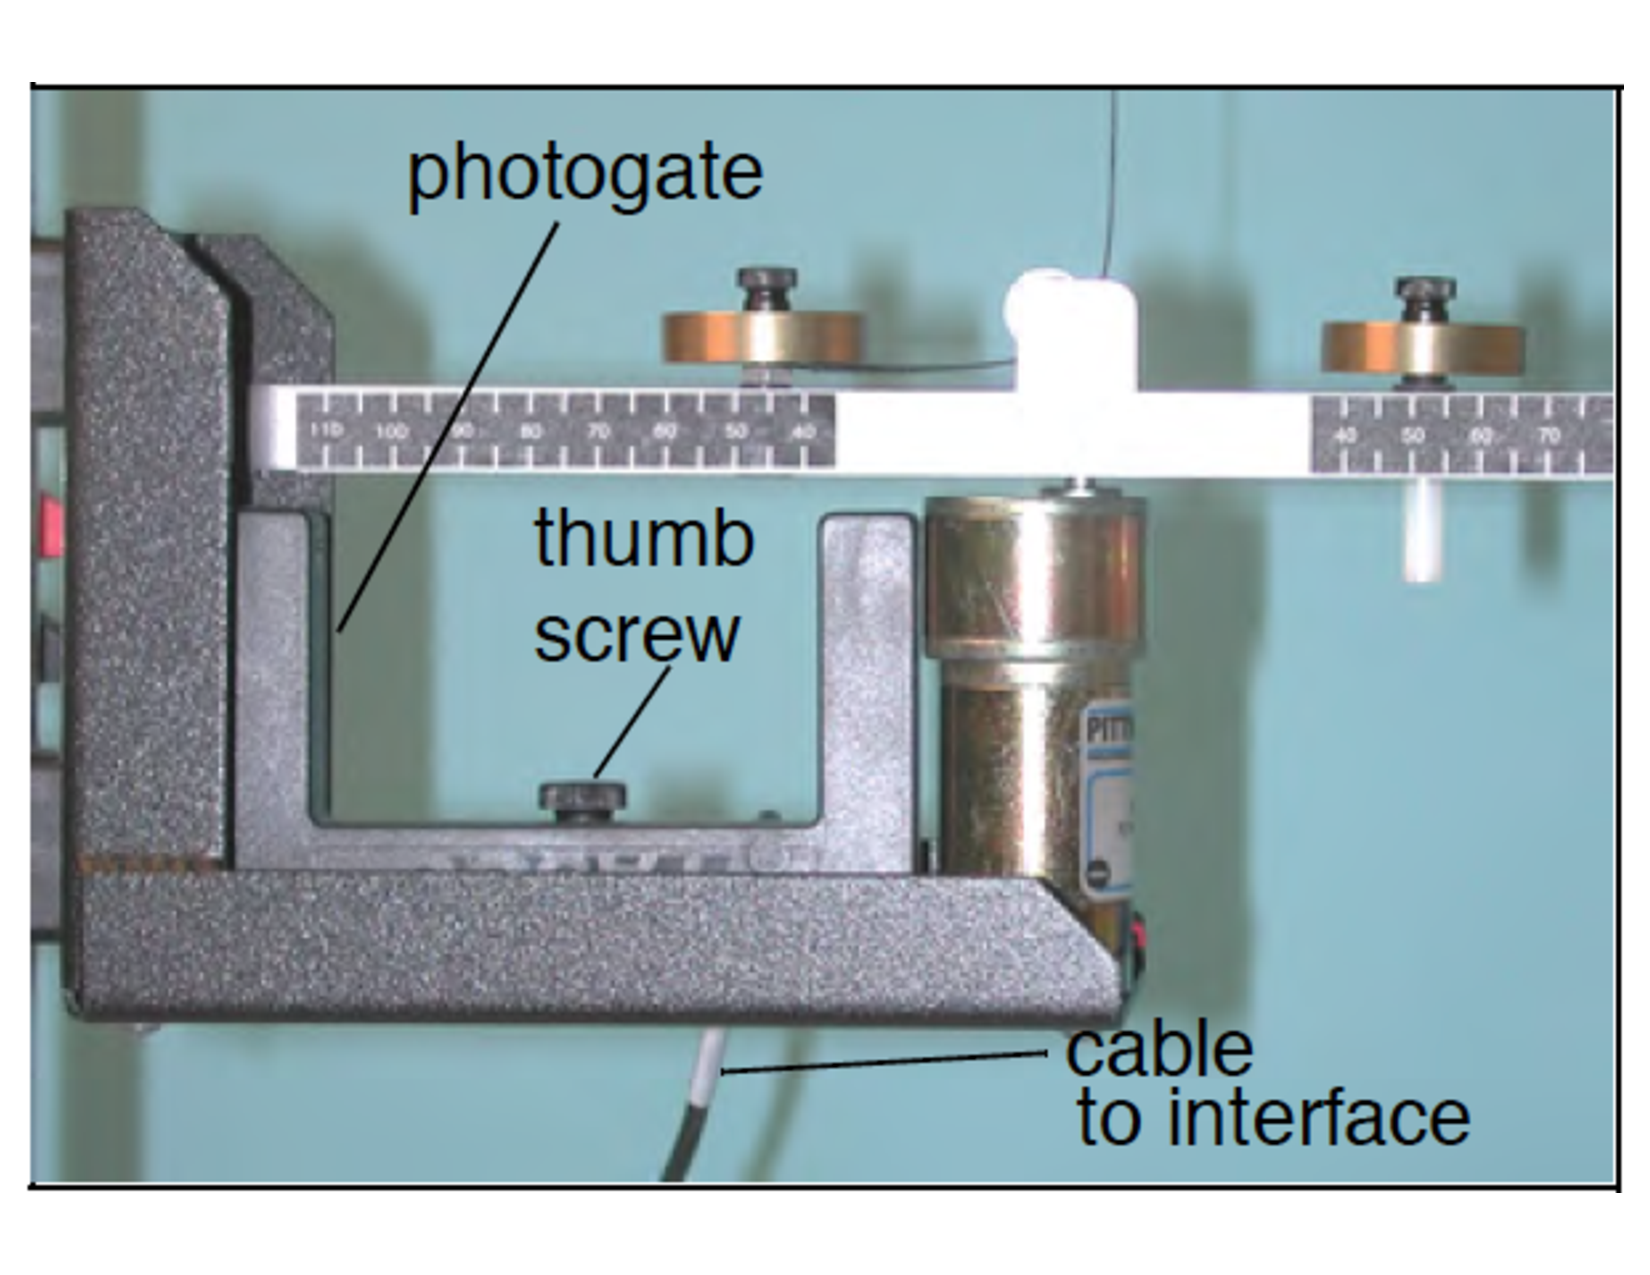
\includegraphics[width=2.9in]{Experiment08Figures/Figure01a.pdf}
    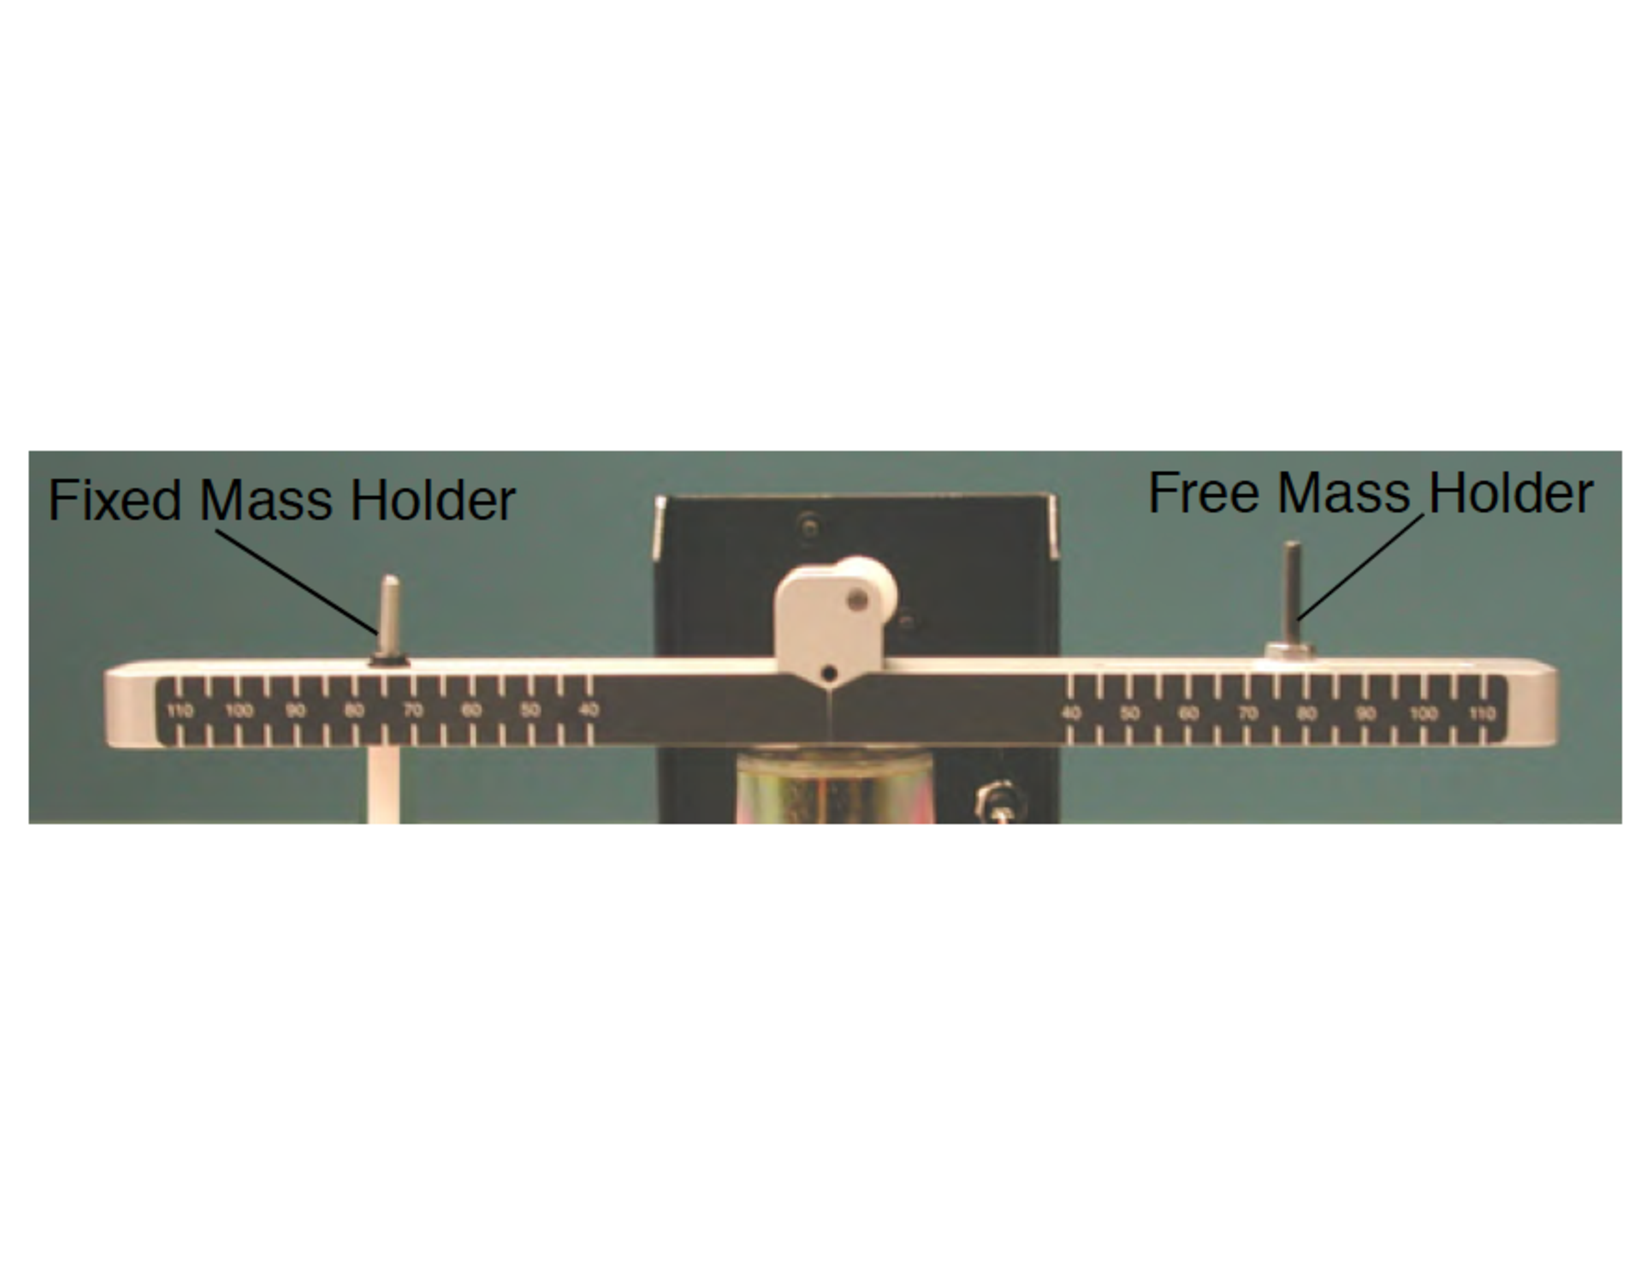
\includegraphics[width=2.9in]{Experiment08Figures/Figure01b.pdf}
  \end{center}
  \caption{Experimental Setup showing the rotating arm and the attached masses. The photogate to measure the speed is shown as well. The small white-ish pin attached underneath one of the mass holders is used to determine the speed $v$ of the mass.}
  \label{M04Fig01}  % the \label command comes AFTER the caption
\end{figure}

In order to determine $v$, the speed of the rotating mass, the rate at which the small pin attached underneath one of the two mass holders will move as it passes through the gap of the photogate is recorded. In order to do so correctly the width of the pin needs to be known to a very high precision.

In this experiment, the force needed to keep the mass at its predetermined radius is measured and plotted against the square of the speed of the mass at the same instant. You will repeat the experiment several times with different masses and at different radii.


\section{Experimental Procedure}

\begin{figure}
  \begin{center}
    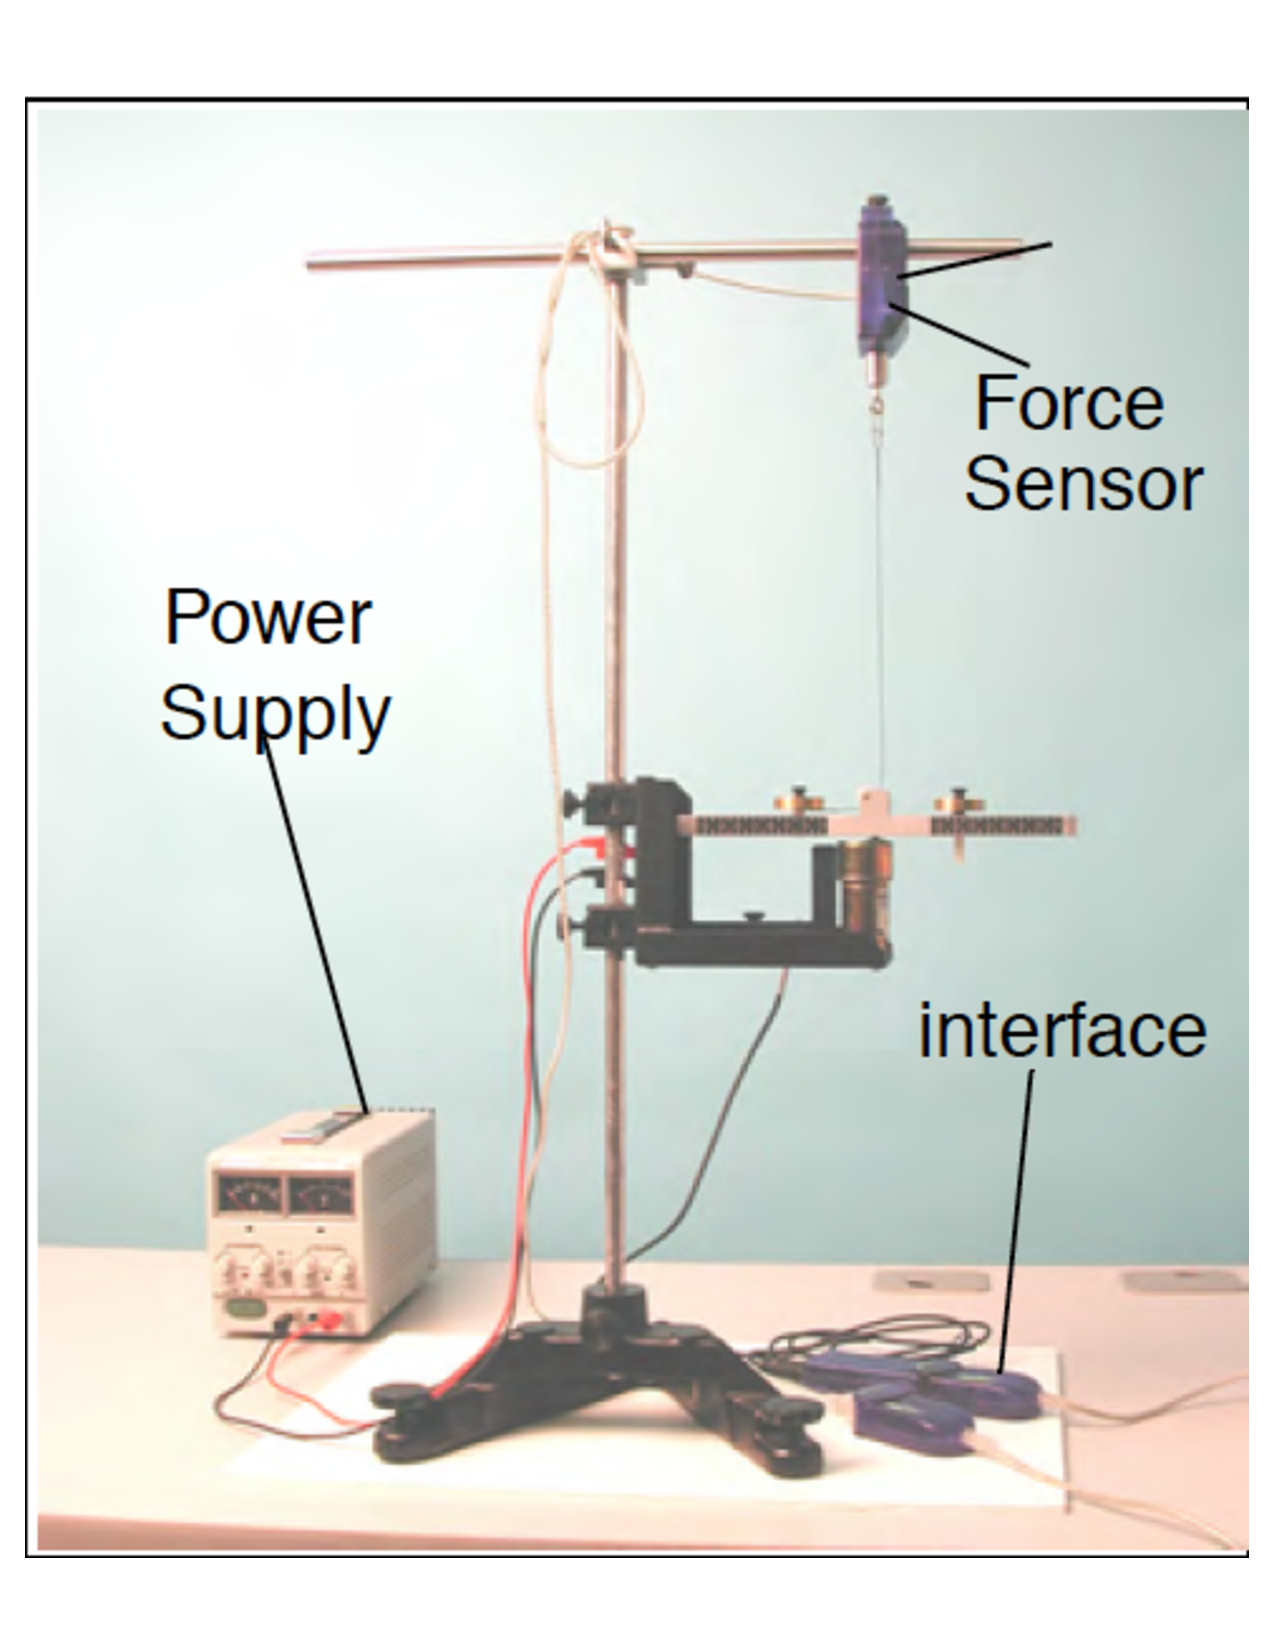
\includegraphics[width=2.6in]{Experiment08Figures/Figure02.pdf}
  \end{center}
  \caption{Experimental Setup for M-\ref{lab:M4}}
  \label{M04Fig02}
\end{figure}

\begin{figure}
  \begin{center}
    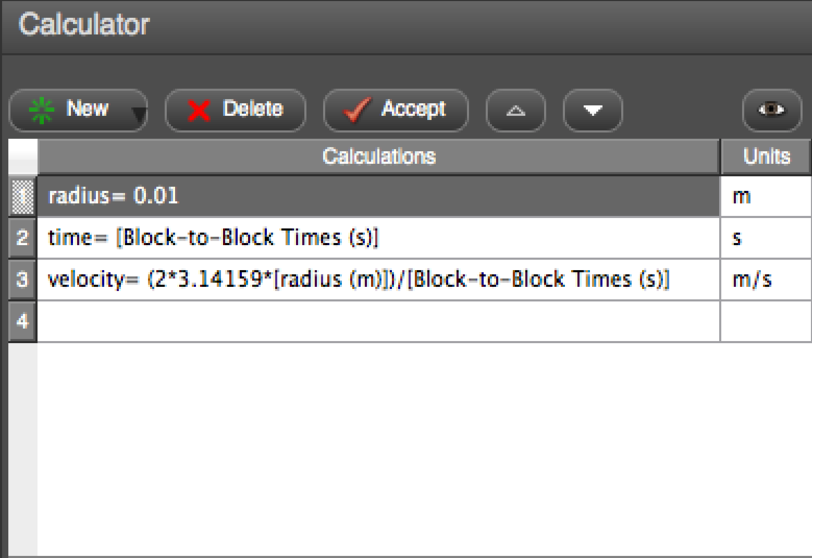
\includegraphics[width=3.3in]{Experiment08Figures/Figure03.pdf}
  \end{center}
  \caption{Setup of the data acquisition system \textbf{Capstone} to measure the speed of the rotating masses. Make sure to adjust the value for the radius in this window to the actual value used in your experimental setup.}
  \label{M04Fig03}
\end{figure}


\begin{itemize}
\item You'll run 6 cases, each with 3 trials:
\begin{itemize}
    \item 2 radii: short, long
    \item 3 different applied masses: 0 g (empty holder), 5 g, 15 g
\end{itemize}

\item[$\triangleright$] The experiment should already be setup for you as shown in Fig.~\ref{M04Fig02} with masses attached to both the fixed and free mass holders. %The force sensor should be  plugged into the computer via a PasPort adapter that connects a USB port on the computer. The photogate should be connected to a digital converter (a rectangular blue box), which has a USB connector on the other end. The USB connector should be connected to the computer.

\item Remove the free mass holder, and measure its mass with a triple-beam balance. Record this in your data sheet. Put the free mass holder back on the rotating arm.

  
%\item[$\triangleright$] Before you start you therefore need to set a few parameters in the \textbf{Capstone} data acquisition system on the computer. %See the page~\ref{sec:SettingUpHardware} for guidance.
%\item[$\triangleright$] Select \textbf{Hardware Setup} in the menu on the left-hand side on the \textbf{Capstone} interface. You should have an image of PasPort connector and the digital converter appear. Leave the PasPort connector alone --- \textbf{Capstone} will set this sensor up on its own.
%\item[$\triangleright$] With the mouse click on one of the two black dots on the image of the digital converter and select the photogate.
%\item[$\triangleright$] Once you have the photogate appear in the image, click on \textbf{Timer Setup}. The program will now guide you through the steps to set up the sensor.
%  \begin{itemize}
%  \item Step 1: Choose \textbf{Pre-configured timer}. Click \textbf{Next}.
%  \item Step 2: Make sure that the photogate is selected with a check mark. Click \textbf{Next}.
%  \item Step 3: Choose the option \textbf{Photogate with Pulley}. Click \textbf{Next}.
%  \item Step 4: Select only \textbf{Block-to-Block Times}. If any other options have a check-marked box, de-selected these options. Click \textbf{Next}.
%  \item Step 5: Leave the defaults ($\mbox{Spoke Arc Length} = 0.015\,\meter$ and $\mbox{Spoke Angle} = 36\degree$) for the two fields. Click %\textbf{Next}.
%  \item Step 6: You may leave the default name of the timer. Click \textbf{Finish}.
%  \end{itemize}
\item[$\triangleright$] Select \textbf{Calculator} in the menu on the left-hand side on the \textbf{Capstone} interface. This will open a window (example shown in Fig.~\ref{M04Fig03}) where you can update the radius to match the actual radius of your masses. \textit{NOTE}: that the value for the radius will change in the experiment, and you need to adjust the value in \textbf{Capstone} when you switch to the new radius.
  
%\item[$\triangleright$] You are now ready to collect data. Close the setup window by clicking on the \textbf{Calculator} button again.

\item[$\triangleright$] After setting the radius in the calculator, close the setup window by clicking on the \textbf{Calculator} button again.
\item[$\triangleright$] There are graphs set up for you in \textbf{Capstone} plotting
\begin{itemize}
    \item $F$ versus $v^2$
    \item $F$ versus $v$
\end{itemize}
\item Before data recording starts
\begin{itemize}
    \item Zero the force sensor with the zero button (physically on the force sensor) while the connecting cable is slack
\end{itemize}
\item[$\triangleright$] Start the data acquisition on \textbf{Capstone} by pressing the \textbf{Record} button.
  You should notice that the program will start to record values.
\item[$\triangleright$] Slowly increase the voltage on the power supply from 0V to 10V over the course of about 30 seconds.
  The metal arm will start to rotate and you will notice the graphs display the data as it is collected.
  Do not exceed 10 V and turn off the data acquisition (by pressing the \textbf{Record} button again) \textbf{before} returning the power supply to zero.
\item[$\triangleright$] Once you have finished your run, fit a line to your $F$ vs. $v^2$ graph.
  Select the fit box.
  In the Curve Fit Editor, lock the intercept $b = 0$.
  Notice the change in $m$ when you lock $b$. Record the slope $m$ in the Data Table.
\item[$\triangleright$] Fit a Quadratic curve to your $F$ vs. $v$ graph.
  Fit the curve $F=A v^2$ by locking B and C to zero. Notice the change in A when you lock B and C.
  Discuss why B and C should be zero. Record A in the Data Table.
\item[$\triangleright$] Repeat the measurement two more times.
  Calculate the average fit parameters for the three runs.
\item[$\triangleright$] Determine $m$, the value of the rotating mass from both graphs and note the result in your data table.
  Explain how you determine the value from your data.
\item[$\triangleright$] Repeat the experiment with two more masses at the same radius $R$.
  Please call for help in setting up the experiment with the new settings.
  Note all results in your data table. Discuss already why you also need to adjust the mass on the fixed mass holder and not just on the free mass holder.
\item[$\triangleright$] Repeat the experiment with the same 3 masses as above at a different radius $R$.
  Note all results in the data table.
\end{itemize}

%\clearpage
\section{Data Analysis}

%\begin{enumerate}
In this experiment, you measure the centripetal force with two different radii and three different applied masses for a total of six cases.
Each case is repeated for three trials.
The curve fitting to determine the mass is performed with the \textbf{Capstone} program.

For each case, construct a table with a row for each trial including:
\begin{itemize}
\item[$\triangleright$] the radius
\item[$\triangleright$] the applied mass plus the mass of the holder as measured earlier
\item[$\triangleright$] fit parameter $A$ from the $F$ vs. $v^2$ (linear fit)
\item[$\triangleright$] the mass determined from the centripetal $F$ vs. $v^2$
\item[$\triangleright$] the difference between the applied mass plus holder and the determined mass from $F$ vs. $v^2$
\item[$\triangleright$] fit parameter $m$ from the $F$ vs. $v$ (quadratic fit)
\item[$\triangleright$] the mass determined from the centripetal $F$ vs. $v$
\item[$\triangleright$] the difference between the applied mass plus holder and the determined mass from $F$ vs. $v$
\item[$\triangleright$] your estimate of the uncertainty in the radius (i.e. $\text{radius} \pm \text{how much?}$)
\item[$\triangleright$] the uncertainty in the mass from the centripetal force due to your estimated radius uncertainty (\textit{Point to consider}: how much does the derived mass change if you change your value for radius in \textbf{Capstone calculator} by the amount of your estimated radius uncertainty?)
\end{itemize}

From the data collected in the six cases you ran, determine the values of the masses $m$, using the given value for the radius $R$, as well as the related uncertainties.

%\end{enumerate}

%\section{Interpretation of Results}
%\begin{itemize}
%\item[$\triangleright$] Give an explanation on why the masses you measured do not agree with the masses of the weights you attached to the free mass holder.
%\item[$\triangleright$] Discuss, first among yourselves and then with your lab instructor what quantity of the experiment you could determine from your data. For your final answer, give an average value of this quantity.
%\item[$\triangleright$] In your report you need to include an answer as to 
%\end{itemize}




% Interpretation of Results
\section{Post-Lab Submission --- Interpretation of Results}
\begin{itemize}
\item Make sure to submit your finalized data table (Excel sheet)
\item Do the graphs display the expected behavior?
\item Discuss your results. Do your experimentally determined masses $\pm$ uncertainty agree with the actual mass of the applied masses plus mass holder?
\item Discuss uncertainties (sources of, how do they affect your final mass values; what would have the largest affect?).
\item What is the precision of your equipment?
\item What are possible systematic errors for today's experiments?
\item Why there should be the same mass on the fixed mass holder as compared to the free mass holder?
\end{itemize}






